%!TEX root = main.tex
\section{Related Work\label{sec:related}}
\begin{figure}[h!]
\centering
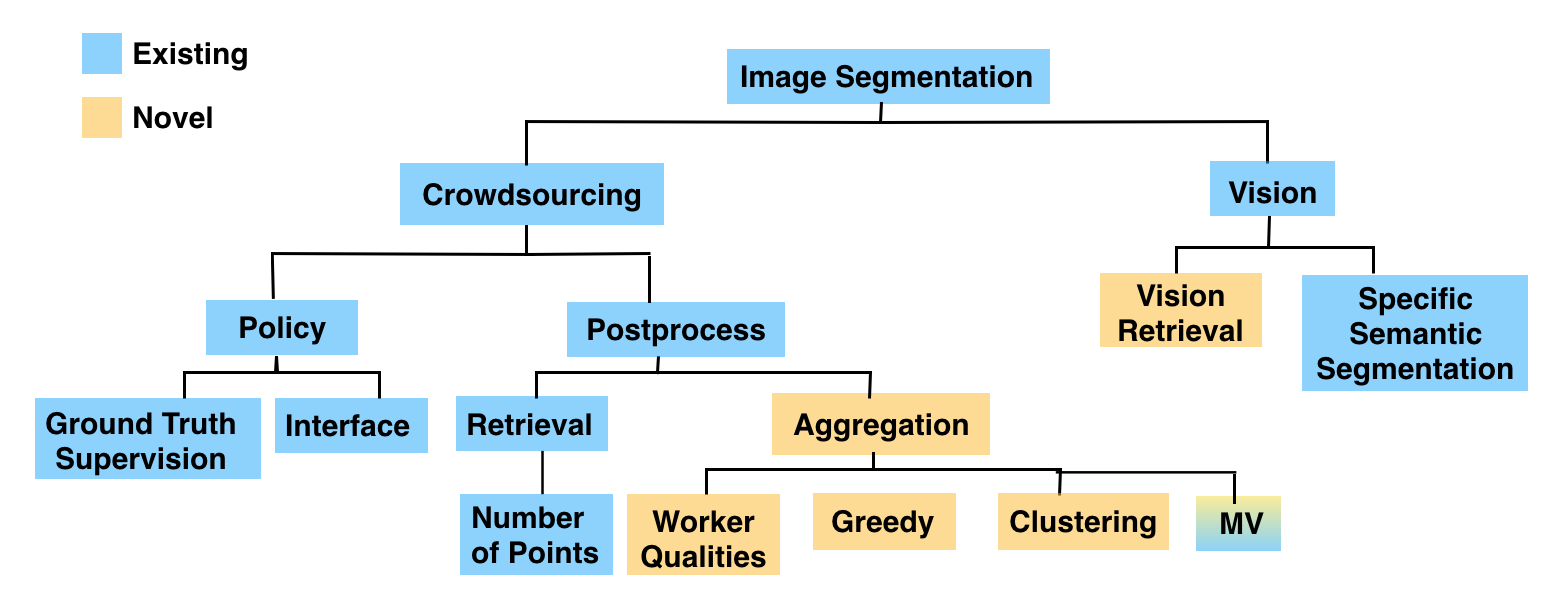
\includegraphics[width=\linewidth]{plots/flowchart.png}
\caption{Flowchart summarizing the classes of existing algorithms for image segmentation (blue) and a novel class of algorithms proposed in this paper (yellow). Majority-vote (MV) is colored both blue and yellow, since a common algorithm in crowdsourcing literature, but have not been extensively applied to crowdsourced image segmentation.}
%The crowdsourced approach can be largely classified as retrieval or aggregation-based methods. We further explore hybrid algorithms that makes use of signals that span over multiple categories, described in our technical report.
\label{flowchart}
\end{figure}
Many large-scale efforts in image segmentation contain little to no information on the quality characterization and evaluation of the collected dataset~\cite{Torralba2010,MartinFTM01,Li2009,Gurari2015}, which indicate the lack of standardized approaches for quality evaluation in crowdsourced image segmentation. As shown in Figure \ref{flowchart}, we break down the existing quality evaluation methods into several categories:
\stitle{Policy-based methods} include specialized segmentation interfaces or workflows that ensures that the data collected are of good quality, including periodic verification workflows~\cite{Lin2014,Everingham15}, specialized segmentation interfaces~\cite{Song2018}, and vision supervision of crowdsourced segmentation\cite{Russakovsky2015,Gurari2016}. %Since these policy-based methods are interface-dependent, require expensive expert-drawn ground-truth annotations or vision information, the results are not easily reproducible. In addition, the segmentations collected by the simple click-and-draw interface in many of the large scale segmentation efforts can not be improved with this technique as a post-processing method. Due to the lack of reproducibility, our paper do not compare against these policy-based methods in extensive details.
\stitle{Retreival-based methods} seek to pick the ``best'' worker segmentation based on some scoring criteria that evaluates the quality of each segmentation, including the use of vision information~\cite{Vittayakorn2011,Russakovsky2015}, expectation-maximization (EM) approaches for bounding box quality estimation~\cite{MDWWelinder2010}, and click-stream behavior\cite{Cabezas2015,Sameki2015,Sorokin2008}.

\stitle{Aggregation-based methods} use multiple worker segmentations to produce a single combined segmentation. %Our paper formulate a novel ``tiles'' approach for aggregation methods that operates on discrete non-overlapping units composed of all worker segmentations overlaid on top of each other. 
Aggregation-based majority vote have been introduced in Sameki et al. (\citeyear{Sameki2015}) as a way for aggregating expert segmentations to obtain a ground truth segmentation for evaluation purposes. 